\mbox{}\\
\vspace{8cm}

This chapter is a reproduction of the following submitted manuscript for publication in GigaScience:

C. I. Mendes, P. Vila-Cerqueira, Y. Motro, J. Moran-Gilad, J. A. Carriço, M. Ramirez. LMAS: Last Metagenomic Assembler Standing

The supplementary information referred throughout the text can be consulted in this chapter before the section of references.

Short-read \ac{SMg} can offer comprehensive microbial detection and characterisation of complex clinical samples. The \textit{de novo} assembly of raw sequence data is key in metagenomic analysis, yielding longer sequences that offer contextual information and afford a more complete picture of the microbial community. The assembly process is the bedrock and may constitute a major bottleneck in obtaining trustworthy, reproducible results.

In this chapter, we present LMAS, an automated workflow developed as a flexible platform to allow users to evaluate traditional and metagenomic dedicated prokaryotic de novo assembly software performance given known standard communities. Its implementation in Nextflow ensures the transparency and reproducibility of the results obtained and the use of Docker containers provides further flexibility. The results are presented in an interactive HTML report where global and reference specific performance metrics can be explored. Currently, 12 assemblers still being maintained are implemented in LMAS, with the possibility of expansion as novel algorithms are developed.

To showcase LMAS we used a test dataset of eight bacterial genomes and four plasmids of the ZymoBIOMICS Microbial Community Standards with linear and logarithmic distribution,  and found that k-mer De Bruijn graph assemblers outperformed the alternative approaches but came with a greater computational cost. Furthermore, assemblers branded as metagenomic specific did not consistently outperform other genomic assemblers in metagenomic samples. Some assemblers still in use, such as ABySS, BCALM2, MetaHipmer2, minia and VelvetOptimiser,  showed significant performance problems and their usability may be limited, particularly when assembling complex samples. 

The performance of each assembler varied depending on the species of interest and its abundance in the sample, with less abundant species presenting a significant challenge for all assemblers. No assembler stood out as an undisputed all-purpose choice for short-read metagenomic prokaryote genome assembly, highlighting that efforts are still needed to further improve metagenomic assembly performance. Our results also suggest that sample complexity and a particular interest in some sample components may affect assembler choice. Using LMAS could help users in their choice of assembler for their specific purpose.  As such, we believe that this manuscript is appropriate for publication in Microbiome as a Software article. 

My contribution to this publication included the design, implementation and optimisation of the LMAS the workflow, including the creation of the Docker containers for all dependencies. I performed the data analysis and comparison of assemblers included in LMAS with ZymoBIOMICS Microbial Community Standards, both evenly and logarithmically distributed samples. Additionally, I've also wrote the manuscript.

\cleardoublepage 

\begin{center}
\large
\textbf{LMAS: Last Metagenomic Assembler Standing}
\end{center}

Catarina I Mendes$^1,*$, 
P Vila-Cerqueira$^1*$,
Y Motro$^2$,
J. Moran-Gilad$^2$,
João A Carriço$^1$
Mário Ramirez$^1$, 


$^1$Instituto de Microbiologia, Instituto de Medicina Molecular, Faculdade de Medicina, Universidade de Lisboa, Lisboa, Portugal 

$^2$Faculty of Health Sciences, Ben-Gurion University of the Negev, Beer-Sheva, Israel

\section{Abstract}

\textbf{Background }The de novo assembly of raw sequence data is key in metagenomic analysis. It allows recovering draft genomes from a pool of mixed raw reads, yielding longer sequences that offer contextual information and provide a more complete picture of the microbial community.

\textbf{Results} To better compare de novo assemblers for metagenomic analysis, LMAS was developed as a flexible platform allowing users to evaluate assembler performance given known standard communities. Overall, in our test datasets, k-mer De Bruijn graph assemblers outperformed the alternative approaches but came with a greater computational cost. Furthermore, assemblers branded as metagenomic specific did not consistently outperform other genomic assemblers in metagenomic samples. Some assemblers still in use, such as ABySS, BCALM2, MetaHipmer2, minia and VelvetOptimiser, perform relatively poorly and should be used with caution when assembling complex samples. 

\textbf{Conclusions} The choice of a de novo assembler depends on the computational resources available, the replicon of interest, and the major goals of the analysis. No single assembler appeared an ideal choice for short-read metagenomic prokaryote replicon assembly, each showing specific strengths. The choice of metagenomic assembler should be guided by user requirements and characteristics of the sample of interest, and LMAS provides an interactive evaluation platform for this purpose. 

\subsubsection{Keywords}

Shotgun Metagenomics, de novo assembly, benchmark, draft genome quality, simulation

\section{Background}

Short-read shotgun metagenomics has the potential to offer comprehensive microbial detection and characterisation of complex clinical or environmental samples.  Despite becoming an increasingly used approach, it comes at the cost of producing massive amounts of data that require expert handling and processing, as well as adequate computational resources. The de novo assembly process is key when analysing metagenomic data since it allows recovering contigs representing the replicons present in the sample, be it genomes, plasmids or bacteriophages, from a pool of mixed raw reads. These contigs are longer sequences that offer better contextual information than reads alone and provide a more complete picture of the microbial community than the species composition. Despite efforts for the development, standardisation and assessment of software for metagenomic analysis, both commercial and open-source \cite{angers-loustau_challenges_2018,gruening_recommendations_2019, sczyrba_critical_2017, couto_critical_2018, meyer_critical_2021}, the de novo assembly process still represents a critical point in these analyses.

The assembly of draft genomes has become a central step when analysing pure bacterial cultures, for instance allowing genomic comparisons through single nucleotide \ac{SNP}s or gene-by-gene methods, such as \ac{cgMLST}. The first assemblers implemented \ac{OLC} approaches, comparing all reads in a sample, computing overlaps and generating consensus sequences by picking the most likely nucleotide for each position in the contigs. As the throughput of sequencing methods increased exponentially, so did the number of pairwise comparisons, limiting the efficiency of these algorithms and making them computationally too expensive. To circumvent this, \ac{dBg} algorithms were increasingly adopted and are currently the most widely used approaches in modern assembly software. Both \ac{OLC} and \ac{dBg} handle unresolvable repeats by essentially fragmenting the sequence, that is, forming multiple contigs for each of the possibly contiguous sequences present in the sample. Additionally, the inherent heterogeneity of complex samples, potentially containing a multitude of replicons, could make traditional genome assemblers, implementing optimisations based on the assumption of having a single genome in the sample, not suitable for metagenomics \cite{ayling_new_2020}.

Several dedicated metagenomic assembly tools for short-read data are available \cite{ayling_new_2020}. These tools are generally assumed to perform better when dealing with complex samples having a combination of intragenomic and intergenomic repeats and uneven and low coverage sequencing depths of some of the replicons \cite{olson_metagenomic_2019}. Not using dedicated metagenomic assemblers was suggested to come with the cost of generating artificial variation and chimeric contigs, especially in samples that contain closely related species \cite{teeling_current_2012}. However, to our knowledge, no formal comparison has been done looking at increased accuracy or gains in contiguity of assemblies obtained with metagenomic assemblers versus traditional assemblers.

With an ever-increasing range of both traditional and metagenomic assemblers becoming available, choosing the best performing tool can be an arduous and time-consuming task since the choice may vary depending on the purpose of the analysis, organism of interest, complexity of the sample and computational infrastructure available. Additionally, the evaluation of the resulting contigs is not straightforward since one metric is not sufficient to classify an assembly, particularly with complex samples \cite{olson_metagenomic_2019,bradnam_assemblathon_2013}. Despite several de novo assembly validation methods relying on features of the created contigs themselves, such as QUAST \cite{gurevich_quast_2013}, being useful in identifying inconsistencies indicative of potential assembly errors, the use of reference-based validation methods offer the possibility of a more complete evaluation of accuracy and are particularly important to benchmark attempts to reconstruct communities. MetaQUAST \cite{bradnam_assemblathon_2013}, a modification of QUAST, extends the original software by performing assembly evaluation based on aligning contigs to a reference, which can be provided or inferred by the software, and reports, in addition to the standard metrics for single genomes reported by QUAST, the number of interspecies translocations and the number of possibly misassembled contigs.

The use of mock communities, with known composition, abundance and genomic information, provides a ground truth against which the success of the assembly of a complex sample can be evaluated. Such mock communities facilitate the identification of misassemblies, such as chimeric sequences generated from the improper combination of two distinct replicons, indels or single nucleotide variants improperly created by the assembler. On the other hand, the comparison of the performance of two assemblers is only possible if the input data is the same and if the same evaluation metrics are applied \cite{sczyrba_critical_2017}. 

To tackle these challenges, we developed LMAS (Last Metagenomic Assembler Standing), an automated workflow to enable the benchmarking of traditional and metagenomic prokaryotic de novo assembly software using defined mock communities. The results of LMAS are presented in an interactive HTML report where selected global and reference replicon specific performance metrics can be explored. The mock communities can be provided by the user to better reflect the samples of interest. New assemblers can be added with minimal changes to the pipeline so that LMAS can be expanded to include novel algorithms as they are developed. The portability and ease of use of LMAS is intended to allow users to evaluate the performance of assemblers in mock communities, mimicking as closely as possible their samples of interest. LMAS is open source and the workflow and its documentation are available at \url{https://github.com/B-UMMI/LMAS} and \url{https://lmas.readthedocs.io/} respectively. 

\section{Implementation}

\subsection{Workflow overview}

LMAS is a user-friendly automated workflow enabling the benchmarking of traditional and metagenomic prokaryotic de novo assembly software using defined mock communities. LMAS was implemented in Nextflow \cite{di_tommaso_nextflow_2017} to provide flexibility and ensure the transparency and reproducibility of the results. LMAS relies on the use of Docker \cite{merkel_docker_2014} containers for each assembler, allowing versions to be tracked and changed easily.

\begin{figure*}[]
\centering
\includegraphics[width=\textwidth]{figures/chapter 5/Figure 1.png}
\caption{The LMAS workflow. The input sequencing data is assembled in parallel, resources permitting, by the set of assemblers included in LMAS. The resulting contigs are processed and the global quality assessment is performed. After filtering for the user-defined minimum contig size, the remaining sequences are mapped against the provided reference and the resulting information is processed to evaluate assembly quality by replicon in the reference file. All results, and optional text information describing the samples, are grouped in the LMAS report.}
\label{fig:chap5_figure1}
\end{figure*}

\subsection{Installation and Usage}

LMAS can be installed through Bioconda \cite{noauthor_lmas_nodate} or Github \cite{mendes_lmas_2021}, with detailed instructions available in the documentation \cite{noauthor_installation_nodate}. LMAS requires as inputs the complete reference replicons (genomes, plasmids or any other replicons present) and short-read paired-end raw data. All complete references (linear replicons) should be provided in a single file. This raw data can be either obtained in silico by creating simulated reads from the reference replicons or sequencing mock communities of known composition. Optionally, information on the input samples in a markdown file can be provided to be presented in the report.

A step-by-step execution tutorial is available at \cite{noauthor_basic_nodate}. Users can customise the workflow execution either by using command-line options or by modifying the simple plain-text configuration files. To make the execution of the workflow as simple as possible, a set of default parameters and directives is provided. A complete description of each parameter is available in Supplemental Material (see Supplemental Material, Workflow parameters), as well as in the documentation \cite{noauthor_parameters_nodate}.  The results are presented in an interactive HTML report, stored in the “report” folder in the directory of LMAS’ execution. The output files of all assemblers and quality assessment processing scripts in the workflow are stored in the “results” folder, in the same location. 

\subsection{Supported Assemblers and selection criteria}

A collection of de novo assembly tools was compiled, including \ac{OLC} and \ac{dBg} assembly algorithms, the latter including both single k-mer and multiple k-mer value approaches, and hybrid assemblers implementing both algorithms, including both genomic and metagenomic assemblers (Supplemental Table S1). Of these, 12 assemblers were selected based on the date of last update and are implemented in LMAS: ABySS \cite{jackman_abyss_2017} (version 2.3.1), BCALM2 \cite{chikhi_compacting_2016} (version 2.2.3), GATB Minia Pipeline \cite{noauthor_gatbgatb-minia-pipeline_2022} (commit hash 9d56f42) , IDBA-UD \cite{peng_idba-ud_2012} (version 1.1.3), MEGAHIT \cite{li_megahit_2015} (version 1.2.9), MetaHipMer2 \cite{georganas_extreme_2018} (version 2.0.0.65-gaad446d-dirty-AddGtest), metaSPAdes \cite{nurk_metaspades_2017} (version 3.15.3), minia \cite{chikhi_space-efficient_2013} (version 3.2.6), SKESA \cite{souvorov_skesa_2018} (version 2.5.0), SPAdes \cite{bankevich_spades_2012} (version 3.15.3), Unicycler \cite{wick_unicycler_2017} (version 0.4.9) and VelvetOptimiser \cite{seemann_velvetoptimiser_2021} (commit hash 092bdee) (Table \ref{tab:ch5_table1}). The execution commands for each assembler are available as Supplemental Material (see Supplemental Material, Short-read de novo assemblers) and in the documentation \cite{noauthor_short-read_nodate}. 
New assemblers can be added with minimal changes to the pipeline so that LMAS can be expanded as novel algorithms are developed. A template is available to facilitate their integration and a step-by-step guide is included in the documentation \cite{noauthor_add_nodate}. The only two requirements for the addition of a new assembler are the execution command for the assembler for paired-end short-read data and a Nextflow-compatible container with the assembler and any dependencies.

\begin{scriptsize}
\begin{center}

\begin{table}[]
\centering
\caption{Prokaryotic de novo assemblers integrated into LMAS.}
\label{tab:ch5_table1}
\begin{tabular}{@{}lll@{}}
\toprule
Assembler         & Type        & Algorithm                        \\ \midrule
GATBMiniaPipeline & Metagenomic & Multiple   k-mer De Bruijn graph \\
IDBA-UD           & Metagenomic & Multiple   k-mer De Bruijn graph \\
MEGAHIT           & Metagenomic & Multiple   k-mer De Bruijn graph \\
MetaHipMer2       & Metagenomic & Multiple   k-mer De Bruijn graph \\
metaSPAdes        & Metagenomic & Multiple   k-mer De Bruijn graph \\
ABySS             & Genomic     & Single   k-mer De Bruijn graph   \\
BCALM2            & Genomic     & Single   k-mer De Bruijn graph   \\
MINIA             & Genomic     & Single   k-mer De Bruijn graph   \\
SKESA             & Genomic     & Multiple   k-mer De Bruijn graph \\
SPAdes            & Genomic     & Multiple   k-mer De Bruijn graph \\
Unicycler         & Genomic     & Multiple   k-mer De Bruijn graph \\
VelvetOptimizer   & Genomic     & Multiple   k-mer De Bruijn graph \\ \bottomrule
\end{tabular}
\end{table}

\end{center}
\end{scriptsize}


\subsection{Assembly Quality Metrics}

The success of an assembly is evaluated in two steps: globally (see \ref{sssec:_chap5_global_metrics}) and relative to each of the replicons present in the sample (see \ref{sssec:_chap5_reference_metrics}). In both, the tabular presentation in the reports allows the comparison of exact values between assemblers, and the interactive plots allow a more intuitive overview and easy exploration of results. In addition to the assembly success metrics, computational resource statistics are registered for each assembler (see Supplemental Material, LMAS Metrics, Computational Performance Metrics).

\subsubsection{Global Metrics} \label{sssec:_chap5_global_metrics} 

The computation of the global metrics is performed through statistics inherent to the complete set of contigs assembled per sample, independent of the species/sample of origin. The metrics are presented, in tabular form, for the complete set of contigs and those filtered for a minimum length, and also graphically for the contigs filtered for a minimum length. The statistics include information on contig number, size and ambiguous bases; and the proportion of reads mapping to the created contigs. Two statistics are a consolidation of per reference metrics: misassemblies (i.e. contigs that do not reflect the structural organisation in the reference replicons); and the overall size of gaps in all reference replicons not covered by any contig. A more detailed description of all global metrics is available in Supplemental Material (see Supplemental Material, LMAS Metrics, Global Metrics). 

\subsubsection{Per Reference Metrics} \label{sssec:_chap5_reference_metrics} 

For the computation of the reference-based metrics, only the \ac{FS} contigs are considered, for each reference replicon in the sample. These contigs are the ones exceeding the user-defined minimum sequence length, filtered using BBTools (version 38.44). After this initial step, the contigs are mapped to the reference replicons with minimap2 \cite{li_minimap2_2018} (version 2.22). The metrics are computed through custom python code (see Supplemental Material, Assembly filtering and mapping) for each replicon in the file provided as input. A detailed description of all reference-based metrics is available in Supplemental Material (see Supplemental Material, LMAS Metrics, Per Reference Metrics). 

In addition to the statistics shared with the global metrics, LMAS also calculates the number of mismatches relative to each reference, the COMPASS \cite{earl_assemblathon_2011} metrics and two new metrics we propose: \ac{LSA} and \ac{Pls}.

\ac{LSA} represents the fraction of the longest single alignment between a contig and the reference, relative to the reference length. The \ac{Pls}, or Phred-like score, is a scoring function based on the identity of each aligned contig to the reference replicon. Similarly to the Phred quality score \cite{ewing_base-calling_1998}, a measure of the quality of the identification of the bases by sequencing, the \ac{Pls} measures the quality of the assembly of a contig. The formula of \ac{Pls} is similar to the Phred score formula but uses as the error function the identity of the base in the contig to that of the reference replicon. The formula to obtain the \ac{Pls} metric per contig is Equation \ref{ch5_eq1}. 

\begin{equation} \label{ch5_eq1}
    Phred(E) = \left\{\begin{matrix}
-log(E)\times 10 & \textup{if }E < 60\\ 
 60 & \textup{if }E = 60
\end{matrix}\right. \\
\textup{ where }E = 1-\textup{Identity}
\end{equation}

\subsection{The LMAS Report}

The LMAS results are presented in an interactive HTML. The LMAS report is composed of two main panels: a top summary panel with information on input samples (provided by the user) and the resources used during LMAS’ execution, and a bottom panel where selected global and reference specific assembly metrics can be explored for each sample. LMAS constructs the HTML file after workflow completion, storing it in the “reports” folder. The report data can be easily shared between users and requires only a browser for visualisation.

\begin{figure*}[h!]
\centering
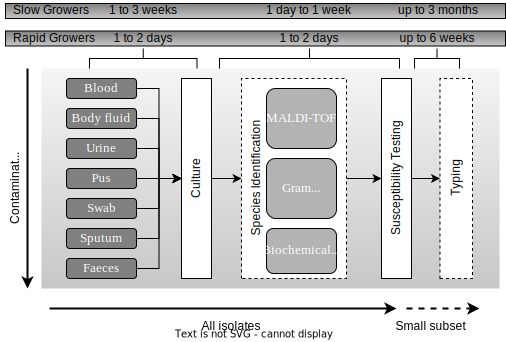
\includegraphics[width=\textwidth]{figures/chapter 5/Figure 2.png}
\caption{The LMAS report.  All results, and optional text information describing the samples, are grouped in the LMAS report, an interactive and responsive HTML file,  for exploration in any browser. Links for LMAS source code and documentation are available in the top right corner of the report. 1) The summary panel of the LMAS report contains information on the input reference sequences and raw sequencing data samples (provided by the user), and the overall computational performance of the assemblers in LMAS. 2) The LMAS metric panel contains the explorable global and reference specific performance metrics per input raw sequencing data sample.  The tabular presentation allows direct comparison of exact values between assemblies, and the interactive plots allow for an intuitive overview and easy exploration of results. 3) If an assembler fails to produce an assembly, or fails to assemble sequences that map to the reference replicon, it is marked in the table with a red warning sign. 4) The global or reference replicon specific metrics can be accessed for each sample in the dropdown menu.}
\label{fig:chap5_figure2}
\end{figure*}

\subsubsection{Summary Panel} \label{sssec:_chap5_summary_panel}

The top panel of the report contains information on the input samples and overall performance of the assemblers in LMAS, divided into three tabs:  Overview, Performance and About us. On the top right corner of the report, direct links to LMAS’ source repository and documentation are provided.

\begin{itemize}
    \item \textit{Overview}: This tab contains information on the input data, including the name and number of reads of the raw sequencing data, and the name of the reference file. Additional information provided by the user about the community used as input is also presented here. 
    \item \textit{Performance}: This tab contains a table with information on the version, the containers used and computational performance metrics for each assembler in LMAS.
    \item\textit{ About us}: This tab contains information on the LMAS GitHub repositories and the LMAS development team. 
\end{itemize}

\subsubsection{Metrics Panel} \label{sssec:_chap5_summary_panel} 

The bottom portion of the report contains the explorable global and reference specific performance metrics per input raw sequencing data sample. Each sample has its own tab and the global or reference replicon specific metrics can be accessed in the dropdown menu. 


\paragraph{Global Metrics} \label{sssec:_chap5_summary_panel_global} \mbox{}\\

A table displays the global assembly metrics computed for the complete and \ac{FS} contigs. If an assembler fails to produce an assembly, it is marked on the table with a red warning sign. The global metric plots are interactive, allow zooming in on particular areas and provide extra information as hover text boxes. The plots can be saved as PNG in whatever view the user selects. 

\paragraph{Per Reference Metrics} \label{sssec:_chap5_summary_panel_reference} \mbox{}\\

Similarly to the global assembly metrics, a table displays the computed set of reference restricted metrics for the \ac{FS} contigs. If an assembler fails to produce sequences that align to the reference, these are marked in the table with a red warning sign. Information on the expected reference replicon length and the GC content is calculated from the input files and reported above the table. The per-reference metric plots are also interactive, allowing the same type of operations as the global metric plots. 

\subsection{Comparison with other assembly evaluation software programs}

The assessment and evaluation of genome assemblies has been a relevant field ever since the emergence of the assembly process itself, and therefore many solutions have been proposed \cite{sczyrba_critical_2017, olson_metagenomic_2019, bradnam_assemblathon_2013, gurevich_quast_2013, mikheenko_metaquast_2016, manchanda_genomeqc_2020, meader_genome_2010, challis_blobtoolkit_2020}. The Critical Assessment of Metagenome Interpretation (CAMI) proposed a set of recommendations and best practices for benchmarking in microbiome research \cite{meyer_tutorial_2021}. These recommendations include the reporting of computational performance, which may condition the choice of software by the users, such as runtime, disk space and memory consumption, also reported by  LMAS (see Supplementary Material, LMAS Metrics). As also suggested by CAMI, LMAS tracks the exact program version and command-line calls through its implementation in Nextflow. Moreover,  using containerised assemblers and being easily installable through Bioconda, LMAS facilitates deployment in diverse user machines. Unlike the CAMI tutorial, in which users are asked to download and install the necessary tools, in LMAS everything is provided in a one-stop reproducible workflow that effortlessly handles all pre-processing, assembly, post-processing, traceability and report production steps, freeing users to focus on providing relevant samples for analysis and interpreting the results in view of the intended applications.

Concerning software for assembly quality assessment currently available, the most widely adopted is QUAST \cite{gurevich_quast_2013}, or when dealing with metagenomic data, its extension metaQUAST \cite{mikheenko_metaquast_2016}, which was also adopted by the CAMI challenges [3,5] \cite{sczyrba_critical_2017, meyer_critical_2021} and suggested in the CAMI Tutorial \cite{meyer_tutorial_2021}. Although several features of these tools overlap with LMAS’ quality assessment components, these differ from LMAS in the sense that they are not a single step workflow allowing a traceable and reproducible assembly of mock communities. Unlike QUAST and metaQUAST, whose purpose is to evaluate assemblies, the purpose of LMAS is to allow users to evaluate assembler performance for a given sample of interest. Supplementary Table S2 shows the comparison of the output and computed assembly quality metrics generated by LMAS, QUAST and metaQUAST. 

\section{Results and Discussion}

To illustrate the use of LMAS and evaluate the performance of the chosen assemblers we used the eight bacterial genomes and four plasmids of the ZymoBIOMICS Microbial Community Standards as reference. As input we used the raw sequence reads of mock communities with an even and logarithmic distribution of species, from real sequencing runs \cite{nicholls_ultra-deep_2019} and simulated read datasets, with and without error, matching the distribution of species in each sample \cite{gourle_simulating_2019}. Our dataset is composed of samples ENN (in silico generated evenly distributed without error), EMS (in silico generated evenly distributed with Illumina MiSeq error model), ERR2984773 (evenly distributed real Illumina MiSeq sample), LNN (in silico generated logarithmically distributed without error), LHS (in silico generated logarithmically distributed with Illumina HiSeq error model) and ERR2935805 (logarithmically distributed real Illumina HiSeq sample) (see Supplemental Table S3). Detailed information about the generation of the input samples is available as Supplemental Material (see Supplemental Materials, ZymoBIOMICS microbial community standards, Supplemental Table S4). To evaluate the reproducibility of an assembler performance, the LMAS workflow was run three times for all samples using default parameters, and the resulting data was processed for each sample (see Supplemental Materials, Assessment of Assembly Success) Supplementary Table S5 to Table S10 present an overview of the average global performance per assembler for each sample in LMAS. 

\subsection{Some assemblers perform poorly}

Of the 12 de novo prokaryotic assemblers included in LMAS, five stand out as having an overall poor performance: ABySS, BCALM2, MetaHipmer2, minia and VelvetOptimiser. Both ABySS and MetaHipmer2 performed inconsistently with differing resource requirements for the same sample in different runs, namely run time and memory allocation (see Supplemental Materials, Resource Requirements Differ Greatly, Supplemental Figure S2).  Moreover, ABySS failed to produce an assembly for sample ERR2984773 for 1 of the runs (see Supplementary Table S7) and for sample LHS in any of the 3 runs in the time limit of 3 days (see Supplementary Table S9), and MetaHipmer2 failed to produce an assembly for samples LNN and LHS in all 3 runs (see Supplementary Tables S8-S9). VelvetOptimiser generated the highest number of inconsistent contigs across the 3 LMAS runs (Figure \ref{fig:chap5_figure3}, Supplementary Table S11), with 1.69\% of the total contigs created present in only 1 or 2 runs. Although not as extreme as VelvetOptimiser, ABySS (0.52\%), minia (0.14\%), GATBMiniaPipeline (0.32\%), MetaHipMer2 (0.11\%) and IDBA-UD (0.08\%) also showed inconsistencies in contig size.

\begin{figure*}[h!]
\centering
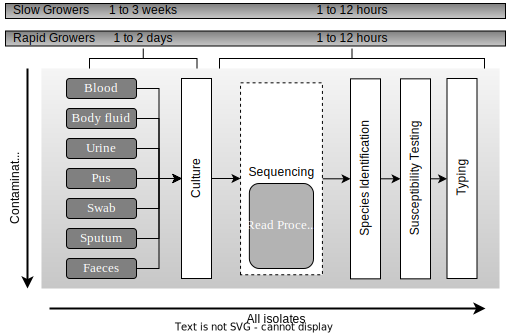
\includegraphics[width=\textwidth]{figures/chapter 5/Figure 3.png}
\caption{Assembly robustness. Inconsistent contigs produced per assembler over 3 LMAS runs. The distribution of contig sizes, in basepairs, consistently present in all three LMAS runs are indicated in the grey boxplots for each assembler. If an assembler produced a contig only present in two of the runs (as determined by its size), its size is indicated in teal. If a contig is present in a single run, it is represented in red.}
\label{fig:chap5_figure3}
\end{figure*}

Regarding the quality assessment of the assemblies produced (Figure \ref{fig:chap5_figure4}, Supplementary Table S12), ABySS, BCALM2 and minia are the only single k-mer \ac{dBg} assemblers in the collection and were found to mostly underperform relative to their multiple k-mer \ac{dBg} counterparts, generally resulting in more fragmented assemblies, although there were significant differences in performance across samples. Among multiple k-mer assemblers, VelvetOptimiser frequently produced a very high number of contigs of very small size (over 99\% of the contigs not surpassing the minimum length of 1,000 \ac{bp}) and therefore a low N50 (an average of 29,768 \ac{bp} versus a global average of 84,114 \ac{bp}) (Supplementary tables S5-S10). Additionally, ABySS and VelvetOptimizer produced contigs with a very large number of Ns, with an average of 1,019 and 3,035 uncalled bases per assembly, respectively. MetaHipMer2, although having overall average metrics in the two evenly distributed mock samples (ENN and EMS, Supplementary Tables S5-S6) where it was able to run successfully, it severely underperformed in the real samples (ERR2984773 and ERR2935805, Supplementary Tables S7 and S10). Generally, the performance scores of the assemblers decreased considerably for the real samples in comparison with the simulated ones, either with or without error. High utilisation of the reads in the dataset is observed for most assemblers, with on average at least 90\% of the reads mapping back to the assembly, except for ABySS, BCALM2, MetaHipMer2 and VelvetOptimiser whose values are in the range of 46-79\%. Despite an overall good performance, SPAdes produced the highest number of misassembled contigs, with an average of 98 and a maximum of 572 (sample ERR2935805, Supplementary Table S10), in comparison to the global average of 11 misassembled contigs for all assemblers across all samples.

Due to their poor performance discussed above, the following assemblers have not been included in subsequent analyses: ABySS, BCALM2, MetaHipmer2, minia and VelvetOptimiser. 

\begin{figure*}[h!]
\centering
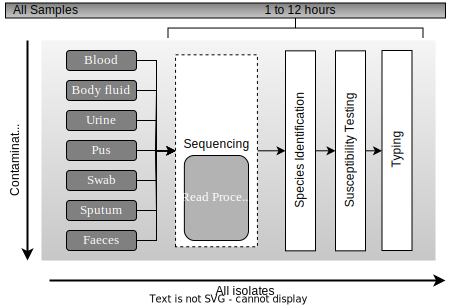
\includegraphics[width=\textwidth]{figures/chapter 5/Figure 4.png}
\caption{Assembler performance for the ZymoBIOMICS Microbial Community Standards dataset. For each sample in the dataset, the best score of each assembler in the 3 LMAS runs was selected. The results for each global assembly metric was normalised, with 1 representing the best result, and 0 the worst. For the original assembly, the following metrics are presented: number of contigs produced (in blue), number of basepairs produced (in teal), the size of the largest contig assembled (in green), N50 (in yellow), percentage of mapped reads to the assembly (in orange) and uncalled bases (in red).  For the filtered assembly, the additional metrics are presented: number of misassembled contigs (in purple) and number of misassembly events (in brown). }
\label{fig:chap5_figure4}
\end{figure*}

\subsection{Metagenomic dedicated assemblers do not outperform genomic assemblers}

After excluding the poorly performing assemblers, LMAS includes 3 genomic (SKESA, SPAdes and Unicycler) and 4 labelled as metagenomic specific (GATBMiniaPipeline, IDBA-UD, MEGAHIT and metaSPAdes) de novo prokaryotic assemblers, all implementing multiple k-mer \ac{dBg} algorithms. As observed in Figure \ref{fig:chap5_figure5}, Supplementary Table S13 and Supplemental Figure S3,  there were very significant differences between the best and the worst performing assemblers of each type, with this difference being more pronounced for metagenomic assemblers. The best performing assemblers of each type behaved frequently quite similarly, and the differences between them tended to be attenuated after filtering for contigs <1 k\ac{bp}. Still, for the linearly distributed samples (ENN, EMS and ERR2984773), the overall worst performers tended to be metagenomic assemblers. In contrast, for the logarithmically distributed samples (LNN, LHS and ERR2935805) the opposite was observed, with genomic assemblers tending to be the worst-performing (Figure \ref{fig:chap5_figure5}). For the logarithmically distributed samples, the number of basepairs recovered is significantly lower than expected from their composition for both genomic and metagenomic assemblers, particularly after filtering (Supplementary Table S13), as contigs representing the less abundant species are not recovered by either type of assemblers (see Assembler performance is influenced by replicon abundance in the sample). For this dataset, the fact that an assembler is branded as genomic or metagenomic does not translate into better or worse performance in dealing with these complex samples, but rather characteristics of the individual assemblers themselves determine their performance.

\begin{figure*}[h!]
\centering
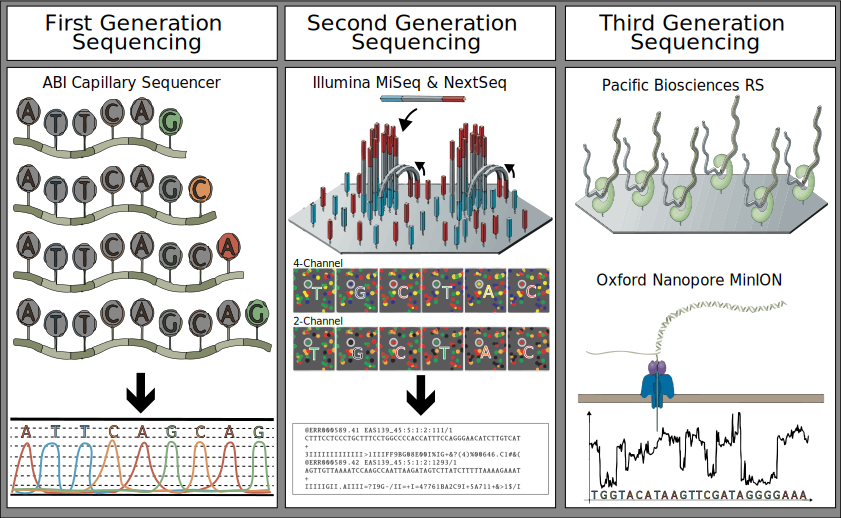
\includegraphics[width=\textwidth]{figures/chapter 5/Figure 5.png}
\caption{Performance of genomic and metagenomic assemblers for the ZymoBIOMICS Microbial Community Standards dataset. For each sample in the dataset and for the 3 runs, the best and worst scores for each assembler category were selected: genomic (in blue) and metagenomic (in red). The results for each global assembly metric were normalised, with 1 representing the best result, and 0 the worst. For the original assembly, the following metrics are presented: number of contigs produced, number of basepairs produced, the size of the largest contig assembled, N50, percentage of mapped reads to the assembly and uncalled bases.  For the filtered assembly, the additional metrics are presented: number of misassembled contigs and number of misassembly events.}
\label{fig:chap5_figure5}
\end{figure*}

\subsection{Success is not straightforward}

Several factors contribute to suboptimal performance of the assembly process, from DNA isolation and library preparation protocol; sequencing technology, depth and read length; to possible contamination and inherent characteristics of the sample composition.

\subsubsection{Assembler performance is influenced by species}

For the eight bacterial genomes present in the samples, even in those with an even distribution of the genomes (ENN, EMS and ERR2984773), variations in the assembly metrics were observed (Figure \ref{fig:chap5_figure6}, Supplemental Figures S4-S6, Supplemental Tables S14-S16).  For all samples in the dataset, the genomes are recovered almost completely, with all replicons being >90\% represented in the resulting assemblies. \textit{Lactobacillus fermentum} is the least represented genome (92.2\%-94.9\%). Most replicon sequences are recovered in <100 contigs, except for \textit{Pseudomonas aeruginosa}, \textit{Escherichia coli} and \textit{Salmonella enterica}, and not considering IDBA-UB, which frequently produces a larger number of contigs when compared to other assemblers. The absolute values of other metrics of assembly quality, such as \ac{LSA}, misassembly events or uncalled bases, are also different between bacterial genomes (Supplemental Tables S14-S16). The fact that \textit{S. enterica} is a closely related species to \textit{E. coli}, with high level of genetic similarity (ANIb >0.8, Supplemental Table S23), could have created difficulties for resolving the assemblies in a mixed sample and lead to the lower coverage observed, the higher number of contigs and the increased number of misassembled contigs identified in these species in some samples. However, in the case of the larger number of contigs of \textit{P. aeruginosa}, no related species are present in the sample and these possibly reflect intrinsic properties of the replicon. Similarly, replicon characteristics could be behind the lower breadth of coverage consistently observed in \textit{L. fermentum} assemblies. 

\begin{figure*}[h!]
\centering
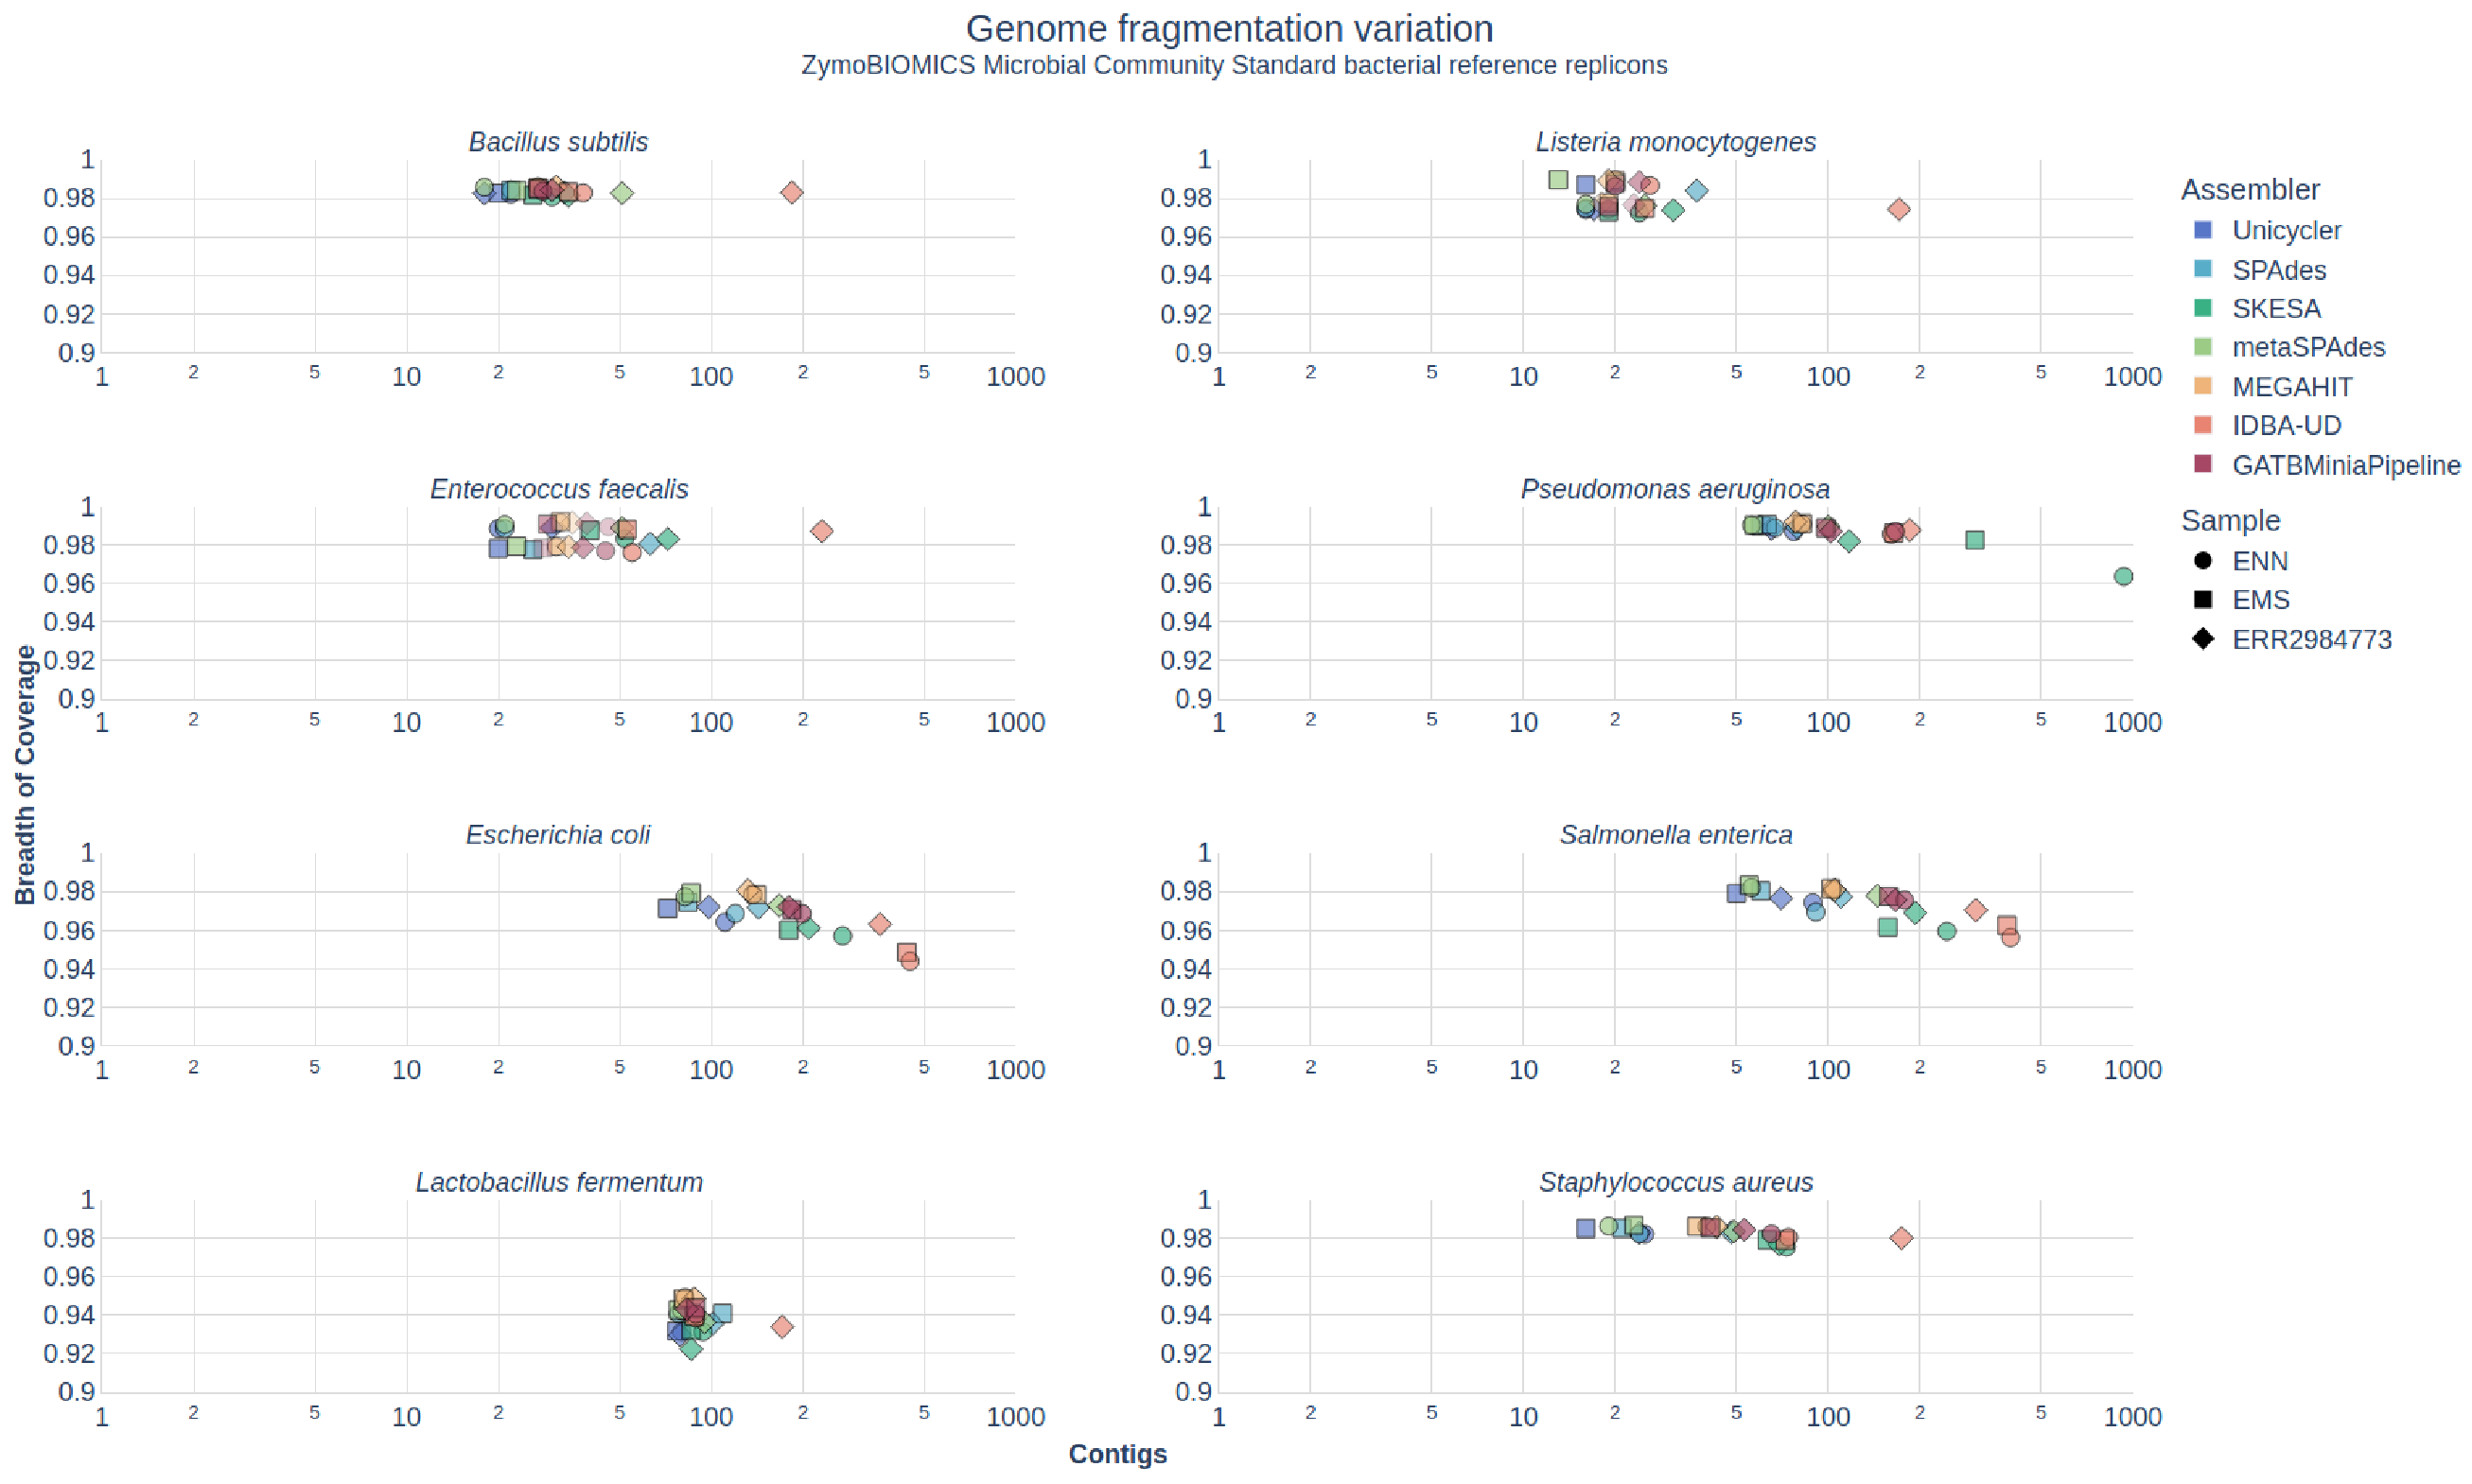
\includegraphics[width=\textwidth]{figures/chapter 5/Figure 6.png}
\caption{Genome fragmentation for each reference replicon of the ZimoBIOMICS community standards dataset for the evenly distributed samples. Genome fragmentation for the 3 LMAS runs is represented by the number of contigs and breadth of coverage of the reference per assembler for the evenly distributed samples: ENN (evenly distributed without error model, identified by a circle), EMS (evenly distributed with Illumina MiSeq error model, identified by a square) and ERR2984773 (real Illumina MiSeq sample, identified by a diamond). Each assembler is identified with the following colour scheme - dark blue: Unicycler, light blue: SPAdes, dark green: SKESA, light green: metaSPAdes, yellow: MEGAHIT, orange: IDBA-UD, red: GATBMiniaPipeline.}
\label{fig:chap5_figure6}
\end{figure*}

\subsubsection{Longer contigs have higher confidence}

The \ac{Pls} metric, which measures the error rate of a contig relative to the reference, shows that for every replicon, longer contigs have higher \ac{Pls} (Figure \ref{fig:chap5_figure7}). This could justify the option of filtering an assembly by length, even beyond the 1000 \ac{bp} minimum contig size implemented by default in LMAS. Not only are we eliminating shorter, less informative contigs in terms of genetic context, but these are also the ones most likely to contain errors relative to the reference sequence. 

\begin{figure*}[h!]
\centering
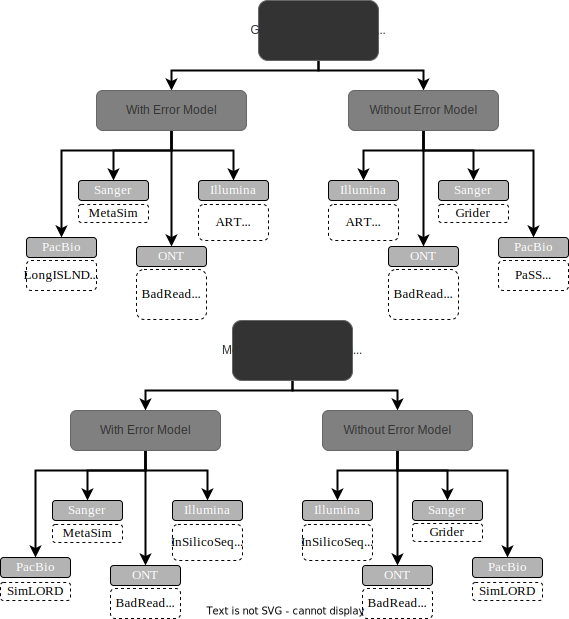
\includegraphics[width=\textwidth]{figures/chapter 5/Figure 7.png}
\caption{: Phred-like score (\ac{Pls}) per contig for each reference replicon of the ZimoBIOMICS community standards datasets. The \ac{Pls} score was calculated for each unique contig produced by each assembler in 3 LMAS runs and is represented in relation to its contig size. Each contig is coloured according to the assembler with the following colour scheme - dark blue: Unicycler,  light blue: SPAdes, dark green: SKESA, light green: metaSPAdes, yellow: MEGAHIT, orange: IDBA-UD, red: GATBMiniaPipeline.}
\label{fig:chap5_figure7}
\end{figure*}

\subsubsection{Longer contigs have higher confidence}

Some genomic regions in several replicons are consistently a challenge for all assemblers. As observed in Figure \ref{fig:chap5_figure8}, all genomes present certain regions that fail to assemble for all tools in all runs, even those generating high-quality draft assemblies. Of all seven assemblers considered, only GATBMiniaPipeline, MEGAHIT and IDBA-UD showed inconsistency in the gaps produced over the 3 LMAS runs (Supplemental Table S17), as expected from producing variable sets of contigs. The regions consistently missing for all assemblers in all runs are rich in repetitive elements, such as rRNA and tRNA coding sequences and mobile genetic elements (Supplemental Table S18), with larger gaps corresponding to tandem sets of these elements. This reflects an intrinsic limitation of short-read sequencing since the length of a read pair is not enough to bridge across the repetitive element, preventing the generation of contigs representing these regions. This is something that could be addressed by the use of long-read sequencing technologies. Despite this, some assemblers are able to produce contigs that represent some of these large tandem regions, such as MEGAHIT and SKESA for \textit{E. faecalis}, and IDBA-UD, MEGAHIT and metaSPADES for \textit{L. monocytogenes}, but such performance is not consistent for all reference replicons. For instance, SKESA fails to assemble two large regions of the \textit{S. enterica} genome that all other assemblers successfully cover.

\begin{figure*}[h!]
\centering
\includegraphics[width=\textwidth]{figures/chapter 5/Figure 8.png}
\caption{Location of gaps in comparison to the reference sequence, per assembler, for each reference replicon of the ZimoBIOMICS community standards datasets. The resulting plot contains the consistent gaps obtained from a three LMAS run for the evenly distributed dataset (ENN, EMS and ERR2984773) for GATBMiniaPipeline, IDBA-UD, MEGAHIT, metaSPAdes, SKESA, SPAdes and Unicycler assemblers.}
\label{fig:chap5_figure8}
\end{figure*}

\subsubsection{Assembler performance is influenced by replicon abundance in the sample}

The logarithmically distributed samples (LNN, LHS and ERR2935805) showed greater variation in the assembly success metrics than the evenly distributed samples (Supplementary Table S8-S10), reflecting the difficulty of recovering sequences of the lowest abundant replicons. For the three replicons with an estimated depth of coverage >15x, a similar pattern is observed in logarithmically distributed samples as in evenly distributed samples, albeit with greater dispersion in the number of contigs generated and with a markedly decreased breath of coverage for some assemblers and samples in the logarithmically distributed samples (Figure \ref{fig:chap5_figure6} and Supplementary Figure S7). Almost no contigs >1000 \ac{bp} were retrieved for replicons with an estimated depth of coverage of <2x resulting in a very low breadth of coverage (<1\%) (Supplementary Table S4, Supplementary Table S22). This leads to a severe underrepresentation of the diversity of the community in the generated contigs, particularly of plasmid sequences due to their smaller length and abundance. This happens despite the greater sequencing depth of these samples versus those with an even distribution (>5-fold difference in the number of reads).

\section{Conclusions}

The purpose of LMAS is to empower users to test assembler performance in meaningful conditions for their experimental setup and objectives. Suitable mock communities, reproducing the users’ samples of interest, can be used as a gold standard to evaluate assembler performance. To illustrate LMAS’ functionalities we analysed a well-known sample used in several studies. Although the eight species ZymoBIOMICS Microbial Community Standards might not be representative of the metagenomic complexity of the samples of interest of most researchers, its relative simplicity means that the results shown probably represent a best-case scenario, since as sample complexity increases so do the challenges to assembler performance. Our results showed significant differences in both global and reference-dependent assembly quality metrics generated by each de novo assembler. The performance of each assembler varied depending on the species of interest and its abundance in the sample, with less abundant species presenting a significant challenge for all assemblers. The fact that an assembler is branded as specific for metagenomics does not guarantee a better performance in metagenomic samples, with assemblers used for genomic assembly outperforming the worst metagenomic assembler tested. The following assemblers showed significant performance problems and their usability may be limited, at least with the default parameters we used: ABySS, BCALM2, MetaHipmer2, minia and VelvetOptimiser.

The choice of de novo assembler depends greatly on the computational resources available, the species of interest, and, possibly, the composition of the community in the sample. In our testing with the ZymoBIOMICS community, no assembler stood out as an undisputed all-purpose choice for short-read metagenomic prokaryotic genome assembly, with different assemblers showing specific strengths. Users would thus benefit from analysing the results of sequencing mock communities or of artificially generated reads simulating their samples of interest to guide their choice of assembler. LMAS was developed to be an easy to use and flexible tool for this purpose. From the results that we obtained with the ZymoBIOMICS dataset, the following assemblers performed consistently well (presented in alphabetical order): MEGAHIT, metaSPAdes, SKESA, SPAdes and Unicycler. From our assessment, we conclude that these assemblers are the most likely candidates to perform well in other complex samples.

LMAS was built with modularity and containerization as keystones, leveraging the parallelization of processes and guaranteeing reproducibility across platforms. The modular design allows for new assemblers to be easily added and existing assemblers to be easily updated, ensuring its future relevance as improvements in assembly software are proposed, and evaluating the gains of such cumulative improvements using the same benchmark set adapted to a specific project or goal. Such reproducibility, capacity to easily add assemblers of interest not included in the current version and flexibility for future extensions are important principles in computational method benchmarking. Moreover, users may compare software performance against mock communities of special interest, depending on their operational focus.

The interactive report provides an intuitive platform for data exploration, allowing the user to easily sift through global and reference specific performance metrics for each sample, as well as providing information on the assemblers executed to allow traceability of the results. Producing an extensive, metric rich report allows users interested in different aspects of assembler performance to make informed decisions, particularly when choosing among the top-performing assemblers, which show only minor differences.

LMAS applies several well-known assembly metrics and proposes two more: \ac{LSA}, which represents the fraction of the longest single alignment between a contig and the reference, and \ac{Pls}, a scoring function based on the identity of each aligned contig to the reference replicon. The entire set of assembly quality metrics used in LMAS allows not only the assessment of quality based on statistics inherent to a set of assembled contigs but also a comparison to a ground truth provided through the use of samples of known composition and reference sequences. The LMAS report provides an interactive and intuitive platform for the exploration of these results, allowing users to easily test assemblers in mock samples with species composition and distribution relevant for their own studies.

Although computationally intensive due to the complex nature of the de novo assembly process, LMAS is the only software integrating assembly and its evaluation into a single pipeline, guaranteeing the same conditions are met for all tools. With LMAS, it is now possible to evaluate which de novo assembler produces the most relevant results for a given community of interest. The LMAS workflow is open-source and its code and documentation are available at https://github.com/B-UMMI/LMAS and https://lmas.readthedocs.io/ respectively.

\section{Availability of supporting source code and requirements}

\textbf{Project name:} LMAS

\textbf{Project home page: }https://github.com/B-UMMI/LMAS 

\textbf{Operating system(s):} UNIX-like systems.
Programming languages: Nextflow, Python, Bash, Javascript

\textbf{Other requirements: }Java version 8 or highest. Docker/Singularity/Shifter

\textbf{License: } GNU GPL v3

\textbf{RRID:} SCR\_022251


\section{Declarations}

\subsection{Ethics approval and consent to participate}

Not applicable.

\subsection{Consent for publication}

Not applicable.

\subsection{Availability of data and material}

The datasets analysed during the current study are available in the Zenodo repository, under \url{https://doi.org/10.5281/zenodo.4588969}. Real sequencing data of the ZymoBIOMICS Microbial Community Standards is available under accessions ERR2984773 and ERR2935805 \cite{nicholls_ultra-deep_2019}. All data generated or analysed during this study are included in this published article, its supplementary information files and the data analysis repository located at \cite{noauthor_lmas_2022}.

\subsection{Competing interests}

MR received honoraria for serving on the speakers' bureau of Pfizer and for consulting for GlaxoSmithKline and Merck Sharp and Dohme. The other authors declare that they have no competing interests. 

\subsection{Funding}

C.I.M. was supported by the Fundação para a Ciência e Tecnologia (grant SFRH/BD/129483/2017).

\subsection{Author’s contributions}

C.I.M., M.R. designed the workflow. C.I.M implemented and optimised the workflow, created the Docker containers, generated mock shotgun metagenomics data used to test and validate the workflow, contributed to the development of the HTML report and analysed the data. C.I.M. and M.R. wrote the manuscript. P.V.C. contributed to the development of the HTML report. M.R., J.A.C. Y.M, and J.M.G critically revised the manuscript.  All authors read, commented on, and approved the final manuscript. 

\subsection{Acknowledgements}

The authors would like to thank Rafael Mamede for his contribution to the implementation and commentary on the several interactive plots implemented throughout the LMAS report. The authors would also like to thank Nabil Fareed-Alikan for his insightful commentary on the interpretation of the results reported in this manuscript, and Anthony Underwood and Robert A. Petit III for their assistance in building the LMAS Nextflow workflow. The author would also like to thank Samuel Nicholls, Joshua Quick, Shuiquan Tang and Nicholas Loman for publicly providing the sequencing data for the ZymoBIOMICS Microbial Community Standards.

\section{Supplemental Materials}

\subsection{Workflow parameters}

In LMAS, a set of default parameters is provided but these can be altered, either by passing the new value when executing the workflow or by editing the “params.config” file in the “configs” folder. There are three main parameters in LMAS: “reference”, “fastq” and “md”. The short-read data is passed as input through the “--fastq” parameter, which by default is set to match all files in the “data/fastq” folder that match the pattern “*\_R{1,2}*”. The reference sequences in a single file can be passed with the “--reference” parameter, matching by default fasta files (with the pattern “*.fasta”) in the “data/reference” folder. Although not mandatory, text information, in a markdown file, on input samples can be passed to LMAS to be presented in the report with the “--md” parameter. By default, this is matched to the “*.md” pattern in the “data” folder.  

Several options are available to alter the behaviour of the assemblers incorporated in LMAS, namely to alter the values of the k-mer for each assembly iteration, as detailed in the documentation \cite{}. By default, these values reflect the corresponding default settings of the assemblers. Additionally, each assembler can be skipped from the workflow, and the resources for the execution, such as CPUs, memory and time limit, can be altered for all assembly processes. For the assembly quality assessment performed by LMAS, the following parameters are provided and can be adjusted: 

\begin{itemize}
    \item “--minLength”: Value for minimum contig length, in basepairs. By default, this value is set to 1000 basepairs;
    \item “--mapped\_reads\_threshold”: Value for the minimum percentage of a read aligning to the contig to be considered as mapped. By default, this value is set to 75\%;
    \item “--n\_target”: Target value for the N, NA and NG metrics, ranging from 0 to 100\%. By default, this value is set to 50\%;
    \item “--l\_target”: Target value for the L metric, ranging from 0 to 100\%. By default, this value is set to 90\%;
\end{itemize}

\subsection{Short-read de novo assemblers}

We have compiled a collection of de novo assembly tools, including \ac{OLC} and \ac{dBg} assembly algorithms, with both single k-mer and multiple k-mer value approaches, and hybrid assemblers (Supplemental Table S1). The collection includes both genomic and metagenomic assemblers, developed explicitly to handle metagenomic datasets. The dates of the last release correspond to the ones available in the preparation of this manuscript.

\subsubsection{Selection Criteria}

Only open-source tools, with clear documentation describing the methodology implemented, were considered. The collection of tools was ordered by the date of the last update, and a Docker container \cite{noauthor_docker_nodate} for the top 12 assemblers was created with the latest released version, with the version used as the tag. In the case of tools where a versioned release is not available, the container was created with the latest version in the default branch of the source repository, using the date of the last update as the tag. The PANDAseq \cite{masella_pandaseq_2012} assembler was excluded due to execution errors. 

\subsubsection{Assemblers in LMAS}

Assemblers benchmarked in LMAS, in alphabetical order:

\paragraph{ABySS} \mbox{}\\

The ABySS assembler \cite{jackman_abyss_2017} is a de novo sequence assembler intended for short paired-end reads and genomes of all sizes. It follows the model of minia, wherein a probabilistic Bloom filter representation is used to encode the de single k-mer size Bruijn graph, reducing memory requirements for de novo assembly. The code is open-source and available at \cite{noauthor_abyss_2022}. The following command is used: “abyss-pe name='\$sample\_id'k=\$KmerSize B=\$BloomSize in='\$fastq”, where “\$sample\_id” contains the identifier of the sample,  contains a list of the input read files, “\$sample\_id” the identifier of the sample, “\$KmerSize” the length of the nodes of the graph (by default set to 96), “\$BloomSize” the size, in Gb, of the bloom filter (by default set to 2 GB), and “\$fastq” the forward and reverse fastq files. 

\paragraph{BCALM2} \mbox{}\\

The BCALM2 assembler \cite{chikhi_compacting_2016} implements a fast algorithm for graph compaction, with low memory requirement, consisting of three stages: careful distribution of input k-mers into buckets, parallel compaction of the buckets, and a parallel reunification step to glue together the compacted strings into unitigs. It’s a traditional single k-mer value dBg assembler. Paired-end information isn’t used, with all given reads contributing to k-mers in the graph. The code is open-source and available at \cite{noauthor_bcalm_2022}. The following command is used: “bcalm -in \$list\_reads -out \$sample\_id -kmer-size \$KmerSize”, where “\$list\_reads” contains a list of the input read files, “\$sample\_id” the identifier of the sample, and “\$KmerSize” the length of the nodes of the graph (by default set to 31). 

\paragraph{GATB-Minia Pipeline} \mbox{}\\

GATB-Minia is an assembly pipeline, still unpublished, that consists of Bloocoo [8] for error correction, minia 3 \cite{chikhi_space-efficient_2013} for contigs assembly, which is based on the BCALM2 assembler \cite{chikhi_compacting_2016}, and BESST \cite{sahlin_besst_2014} for scaffolding. It was developed to extend the minia assembler to use the dBg algorithm with multiple k-mer values and to explicitly handle metagenomic data. The code is open-source and available at \cite{noauthor_gatbgatb-minia-pipeline_2022}. The following command is used: “gatb -1 \$fastq\_pair[0] -2 \$fastq\_pair[1] --kmer-sizes \$kmer\_list -o \$sample\_id”, where \$fastq\_pair[0] contains the forward-facing reads, \$fastq\_pair[1] the reverse-facing reads, \$kmer\_list the list of values for length of the nodes of the dBg (by default set to 21,61,101,141,181), and “\$sample\_id” the identifier of the sample. 

\paragraph{IDBA-UD} \mbox{}\\

IDBA-UD \cite{peng_idba-ud_2012} is a dBg graph assembler for assembling reads from single-cell sequencing or metagenomic sequencing technologies with uneven sequencing depths. It employs multiple depth relative thresholds to remove erroneous k-mers in both low-depth and high-depth regions. The technique of local assembly with paired-end information is used to solve the branch problem of low-depth short repeat regions. To speed up the process, an error correction step is conducted to correct reads of high-depth regions that can be aligned to high confidence contigs. The code is open-source and available at \cite{peng_loneknightpyidba_2022}. The following command is used:  “idba\_ud -l \$fasta\_reads\_single”, where \$fasta\_reads\_single contains the combined sequence data converted to FASTA format reads with “reformat.sh” from BBtools \cite{bushnell_bbmerge_2017}. 

\paragraph{MEGAHIT} \mbox{}\\

MEGAHIT \cite{li_megahit_2015} is a de novo assembler for large and complex metagenomics datasets. It makes use of the succinct dBg, with a multiple k-mer size strategy. In each iteration, MEGAHIT cleans potentially erroneous edges by removing tips, merging bubbles and removing low local coverage edges, especially useful for metagenomics which suffers from non-uniform sequencing depths. The code is open-source and available at \cite{li_megahit_2022}. The following command is used: “megahit -o megahit --k-list \$kmers -1 \$fastq\_pair[0] -2 \$fastq\_pair[1]”, where \$kmers contains the list of values for length of the nodes of the dBg (by default set to 21,29,39,59,79,99,119,141), \$fastq\_pair[0] contains the forward-facing reads, and \$fastq\_pair[1] the reverse-facing reads.

\paragraph{MetaHipMer2} \mbox{}\\

MetaHipMer2 \cite{georganas_extreme_2018} is a  multiple k-mer size dBg de novo metagenome short-read assembler built to run efficiently on both single servers and on multi-node supercomputers, where it can scale up to coassemble terabase-sized metagenomes. The code is open-source and available at \cite{noauthor_berkeleylab_nodate}. The following command is used: “mhm2.py -k \$kmers -r \$fasta\_reads\_single -s 0”, where \$kmers contains the list of values for length of the nodes of the dBg (by default set to “21,33,55,77,99”), where \$fasta\_reads\_single contains the combined sequence data converted to FASTA format reads with “reformat.sh” from BBtools \cite{bushnell_bbmerge_2017}. The “-s 0” option skips the scaffolding step. 

\paragraph{metaSPAdes} \mbox{}\\

SPAdes [19] started as a tool aiming to resolve uneven coverage in single-cell genome data, with metaSPAdes \cite{nurk_metaspades_2017} later released building a specific metagenomic pipeline on top of SPAdes. It uses multiple k-mer sizes of dBg, starting with the lowest kmer size and adding hypothetical k-mers to connect the assembly graph. The code is open-source and available at \cite{noauthor_spades_nodate}. The following command is used: “metaspades.py --only-assembler -k \$kmers -1 \$fastq\_pair[0] -2 \$fastq\_pair[1]”, where \$kmers contains the list of values for length of the nodes of the dBg (by default set to “auto”), \$fastq\_pair[0] contains the forward-facing reads, and \$fastq\_pair[1] the reverse-facing reads.

\paragraph{minia} \mbox{}\\

Minia \cite{chikhi_space-efficient_2013} performs the assembly on a data structure based on unitigs produced by the BCALM \cite{chikhi_compacting_2016} software and using graph simplifications that are heavily inspired by the SPAdes assembler \cite{bankevich_spades_2012}. Minia is a short-read traditional assembler based on dBg graph using a single k-mer length. The code is open-source and available at  \cite{noauthor_minia_2022}. The following command is used: “minia -in \$list\_reads -out \$sample\_id”,  where “\$list\_reads” contains a list of the input read files and “\$sample\_id” the identifier of the sample.

\paragraph{SKESA} \mbox{}\\

SKESA \cite{souvorov_skesa_2018} is a de novo sequence read assembler that is based on dBg and uses conservative heuristics. It is designed to create breaks at repeat regions in the genome, creating shorter assemblies but with greater sequence quality. It tries to obtain good contiguity by using multiple k-mers longer than mate length and up to insert size. The code is open-source and available at \url{https://github.com/ncbi/SKESA}. The following command is used: “skesa --use\_paired\_ends --contigs\_out \$sample\_id --fastq \$fastq\_pair[0] \$fastq\_pair[1]”, where “\$sample\_id” refers to the identifier of the sample, \$fastq\_pair[0] contains the forward-facing reads, and \$fastq\_pair[1] the reverse-facing reads.

\paragraph{SPAdes} \mbox{}\\

SPAdes \cite{bankevich_spades_2012} is an assembly tool aiming to resolve uneven coverage in single-cell genome data through multiple k-mer sizes of dBgs. It starts with the smallest k-mer size and adds hypothetical k-mers to connect the graph. The code is open-source and available at \cite{noauthor_spades_nodate}. The following command is used:  “spades.py --only-assembler -k \$kmers -1 \$fastq\_pair[0] -2 \$fastq\_pair[1] ”, where \$kmers contains the list of values for length of the nodes of the dBg (by default set to “auto”), \$fastq\_pair[0] contains the forward-facing reads, and \$fastq\_pair[1] the reverse-facing reads.

\paragraph{UNICYCLER} \mbox{}\\

Unicycler \cite{wick_unicycler_2017} is an assembly pipeline for bacterial genomes that can do long-read assembly, hybrid assembly and short-read assembly. When assembling Illumina-only read sets, it functions as a SPAdes-optimiser, using a  dBg algorithm with multiple k-mer values. The code is open-source and available at \cite{wick_unicycler_2022}]. The following command is used: “unicycler -o . --no\_correct --no\_pilon -1 \$fastq\_pair[0] -2 \$fastq\_pair[1]”, where \$fastq\_pair[0] contains the forward-facing reads, and \$fastq\_pair[1] the reverse-facing reads.

\paragraph{VELVETOPTIMIZER} \mbox{}\\

This optimising pipeline of the Velvet assembler \cite{zerbino_velvet_2008} is still unpublished but extends the original tool by performing several dBg assemblies with variable k-mer sizes. It searches a supplied hash value range for the optimum, estimates the expected coverage and then searches for the optimum coverage cutoff. It uses Velvet’s internal mechanism for estimating insert lengths for paired-end libraries.  The code is open-source and available at \cite{seemann_velvetoptimiser_2021}. The following command is used: “VelvetOptimiser.pl -v -s \$velvetoptimizer\_hashs -e \$velvetoptimizer\_hashe -f '-shortPaired -fastq.gz -separate \$fastq\_pair[0] \$fastq\_pair[1]'”, where \$velvetoptimizer\_hashs is the lower end of the hash value range that the optimiser will search for the optimum (default: 19), \$velvetoptimizer\_hashe is the upper end of the hash value range that the optimiser will search for the optimum (default: 31), \$fastq\_pair[0] contains the forward-facing reads, and \$fastq\_pair[1] the reverse-facing reads.

\subsection{Misassembly detection} \label{chap5_sup_misassembly}

For the detection of misassembly events in the assemblies, the assembled sequences are first filtered for a minimum sequence length with BBTools \cite{bushnell_bbmerge_2017} (version 38.44), as defined in the parameters, using the following command: “reformat.sh in=\$assembly out=filtered\_\$assembly minlength=\$minLen”, where \$assembly contains the file with the assembled sequences and \$minLen the value of the minimum sequence length allowed. 

The filtered assembled sequences are mapped against the tripled reference replicons, ensuring that the assembled contigs can fully align regardless of their starting position relative to that of the provided reference sequence. This is done with minimap2 \cite{li_minimap2_2018} (version 2.22) with the following parameters: “minimap2 --cs -N 0 -t -r 10000 -g 10000 -x asm20 --eqx”.

\subsection{Assembly filtering and mapping}

The assembled sequences are first filtered for a minimum sequence length with BBTools [14] (version 38.44), as defined in the parameters, using the following command: “reformat.sh in=\$assembly out=filtered\_\$assembly minlength=\$minLen”, where \$assembly contains the file with the assembled sequences and \$minLen the value of the minimum sequence length allowed. 

The filtered assembled sequences are mapped against the tripled reference replicons, as explained above, with minimap2 \cite{li_minimap2_2018} (version 2.22) with the following parameters: “minimap2 --cs -N 0 -t -r 10000 -g 10000 -x asm20 --eqx”.

\subsection{LMAS Metrics}

The following metrics are computed by the LMAS workflow, globally for characteristics intrinsic to the assembled contigs, and relative to the replicons present in the sample. 

\subsubsection{Global Metrics}

\paragraph{General contig information} \mbox{}\\

The following metrics are computed and presented in tabular form: 

\begin{itemize}
    \item \textbf{Contigs:} The total number of contigs in the assembly;
    \item \textbf{Basepairs:} The total number of bases in the assembly;
    \item \textbf{Maximum sequence length:} The length of the largest contig in the assembly;
    \item \textbf{Number of ‘N’s:} Number of uncalled bases;
    \item \textbf{Mapped reads:} Percentage of mapped reads to the assembly;
\end{itemize}

For each plot, the following metrics are presented:

\begin{itemize}
    \item \textbf{Contig size distribution per assembler:} For each assembler in LMAS, a boxplot is computed representing the size distribution of contigs that align to any of the reference replicons. The unmapped contigs, if present, are represented in a red scatterplot overlapping the boxplot. 
    \item \textbf{Gap size distribution per assembler:} For each assembler in LMAS, a boxplot is computed representing the distribution of gap sizes. Gaps are calculated after aligning all contigs to the reference replicons. All gaps ≥1 basepair in length are considered. 
\end{itemize}

\paragraph{Contiguity} \mbox{}\\

The following metrics are computed and presented in tabular form:

\begin{itemize}
    \item \textbf{Nx (where 0  < x  $\leq$ 100):} Length for which the collection of all contigs of that length or longer in an assembly covers at least a given percentage of the total length of the assembly
\end{itemize}

\paragraph{Misassemblies} \mbox{}\\

A misassembly event is defined as a continuously assembled contig being broken into multiple non-collinear blocks when mapping to the reference replicons, i.e. the contig produced by the assembler does not preserve the exact synteny observed in the reference replicon. This may reflect the addition or deletion of sequence stretches or the shuffling of sequence blocks relative to the reference replicons. For a large insertion or deletion to be considered it must be $\geq $50 basepairs in length \cite{kosugi_comprehensive_2019}. This metric is computed for the filtered set of contigs, i.e. those of length above a user-specified minimum size and mapping to the reference replicons (see \ref{chap5_sup_misassembly}). The misassemblies are processed with custom python code. 

The following misassembly types are identified:

\begin{itemize}
    \item \textbf{Chimera:} a contig has two or more sequence blocks mapping to different reference replicons;
    \item \textbf{Insertion:} a sequence block ($\geq $50 basepairs) which is not present in any of the reference replicons has been introduced into the contig by the assembly process;
    \item \textbf{Deletion:} a sequence block ($\geq $50 basepairs) of the reference replicon is missing from the contig created by the assembly process;
    \item \textbf{Inversion:} a contig has at least two sequence blocks mapping to the same replicon but reversed end to end, i.e. one of the blocks maps to the sense strand and the other to the antisense strand in the reference replicon while both are in the same strand in the contig, or vice-versa;
    \item \textbf{Rearrangement:} a contig has at least two sequence blocks mapping to the same replicon, in the same orientation, in a different order than in the reference sequence;
    \item \textbf{Translocation:} a contig has at least two sequence blocks abutting in the contig but mapping non-collinearly (over 1000 base pairs apart) in the reference replicon;
    \item \textbf{Duplication:} a sequence block of a contig maps at least twice to the reference replicon in different alignment blocks;
    \item \textbf{Inconsistency:} a contig has at least two sequence blocks abutting in the contig but fails to be classified in any of the previous categories.
\end{itemize}

Figure \ref{fig:chap5_sup_figure_1} provides a visual description of the detected misassemblies. The following metric is computed and presented in tabular form:

\begin{itemize}
    \item \textbf{Misassembled contigs:} Number of contigs with misassembly events
    \item \textbf{Misassembly events:} Total number of misassemblies in the contigs
\end{itemize}

In the plot, the metrics are presented for the filtered set of contigs:

\begin{itemize}
    \item \textbf{Misassembled contigs:} Scatter plot for misassembled contigs per assembler, the size of the misassembled contigs, and the number of blocks created by the misassembly in the contig.  The distribution of contig size for all misassembled contigs is represented in a boxplot. Information on the misassembly is presented as a hover text for each misassembly event.
\end{itemize} 

\begin{figure*}[]
\centering
\includegraphics[scale=0.95]{figures/chapter 5/Supplemental Figure 1.png}
\caption{LMAS misassembly classification. Misassembled contigs are classified into 6 main categories: chimera, insertion, deletion, inversion, rearrangement, translocation and duplication, according to the mapping orientation, the distance between blocks in the contig and the mapping coordinates in the reference replicon. If a contig is classified as being chimeric, no further classification is performed. The other categories are classified independently of each other, with combinations being possible, to better reflect the differences in comparison to the reference. If a contig is broken into multiple sequence blocks but fails to be classified in any of the previous categories, it is reported as being inconsistent}
\label{fig:chap5_sup_figure_1}
\end{figure*}

\subsubsection{Per Reference Metrics}

\paragraph{General contig information} \mbox{}\\

The following metrics are computed and presented in tabular form: 

\begin{itemize}
    \item \textbf{Contigs:} The total number of contigs in the assembly that align to the reference replicon;
    \item \textbf{Basepairs:} The total number of bases in the assembly that align to the reference replicon;
    \item \textbf{Number of ‘N’s:} Number of uncalled bases (N's) in the contigs that align to the reference replicon.
\end{itemize}

\paragraph{COMPASS} \mbox{}\\

A measure of the quality of a replicon assembly can be considered the proportion of the reference covered by the contigs, i.e. the breadth of coverage of the reference replicon. The COMPASS metrics \cite{bradnam_assemblathon_2013} complement our view of the quality of the assembly with other metrics such as how much redundancy is there in the assembly or the parsimony of the contigs relative to the reference. COMPASS is composed of the following metrics, presented in tabular form:

\begin{itemize}
    \item \textbf{Breadth of Coverage:} Ratio of covered sequence on the reference by aligned contigs;
    \item \textbf{Multiplicity:} Ratio of the length of the alignable assembled sequence to covered sequence on the reference;
    \item \textbf{Validity:} Ratio of the length of the alignable assembled sequence to total basepairs in the aligned contigs;
    \item \textbf{Parsimony:} Cost of the assembly (multiplicity over validity);
\end{itemize}

Additionally, the Breadth of Coverage metric is displayed graphically:

\begin{itemize}
    \item \textbf{Genome Fragmentation:} Scatter plot representing the number of contigs per breadth of coverage of the reference, per assembler.
\end{itemize}

\paragraph{Contiguity} \mbox{}\\

To supplement the traditional NA and NG contiguity metrics implemented in QUAST \cite{gurevich_quast_2013}, we define the LSA metric as the longest single alignment between the assembly and the reference replicon, relative to the reference replicon length, as proposed previously \cite{wick_benchmarking_2021}. This provides a simpler picture of assembly quality as lower contiguity immediately suggests a higher fragmentation, missing sequences or more misassemblies. The following metrics are presented in tabular form:


\begin{itemize}
    \item \textbf{LSA:} longest single alignment between the assembly and the reference, relative to the reference length;
    \item \textbf{NAx (where 0  < x  $\leq$ 100):} Length for which the collection of aligned contigs of that length or longer in an assembly covers at least a given percentage of the total length of the reference replicon;
    \item \textbf{NGx (where 0  < x  $\leq$ 100):} Length for which the collection of aligned contigs of that length or longer covers at least a given percentage of the sequence of the reference.
    \item \textbf{Lx (where 0  < x  $\leq$ 100):} Minimal number of contigs that cover x \% of the sequence of the reference;
\end{itemize}

The NAx, NGx and Lx metrics are presented graphically in a line plot for each value of x, where x represents the percentage of the sequence of the reference, ranging from 0 to 100, per assembler.  

\paragraph{Identity} \mbox{}\\

The identity is defined as the number of exact matches between the contigs and the reference replicon, relative to the reference replicon length. The following metrics are presented in tabular form:

\begin{itemize}
    \item \textbf{Identity:} Ratio of identical basepairs in all aligned contigs to the reference;
    \item \textbf{Lowest identity:} Identity of the lowest scoring contig to the reference;
\end{itemize}

For each plot, the metrics are presented for the contigs filtered for a minimum length that align with the reference replicon.

\begin{itemize}
    \item \textbf{Pls Metric:} Scatter plot for the Phred-like score per contig, per assembler;
    \item \textbf{Gaps: }Location of gaps in comparison to the reference sequence, per assembler, with the cumulative number of gaps per position in the reference. Gaps with 1 basepair or more in length are considered;
    \item \textbf{SNPs:} Location of substitutions in comparison to the reference sequence, per assembler, with the indication of the substitution type and coordinate in the reference. Additionally, the cumulative number of SNPs per position in the reference is presented.
\end{itemize}

\paragraph{Misassembly} \mbox{}\\

Similar to what is performed in Global Metrics, this metric is computed for the filtered set of contigs. An aligned contig is considered misassembled when broken into multiple blocks when mapping to the linear reference replicon. Chimeric contigs aligning to more than one reference replicon are counted in each reference individually. 

\begin{itemize}
    \item \textbf{Misassembled contigs:} Number of aligned contigs that contain a misassembly event;
    \item \textbf{Misassembly events:} Total number of misassemblies in the aligned contigs;
\end{itemize}

Additionally, the following information is shown graphically:

\begin{itemize}
    \item \textbf{Misassemblies:} Location of the alignment blocks of misassembled contigs in comparison to the reference sequence, per assembler, with the cumulative number of basepairs in the alignment blocks per position in the reference.
\end{itemize}

\subsubsection{Computational Performance Metrics}

Different software, implementing distinct de novo assembly algorithms, have distinct computational requirements. As such, computational statistics are registered for each assembler. The following metrics are presented in tabular form:

\begin{itemize}
    \item \textbf{Avg Time:} Average run-time formatted as “hour:minute:second”;
    \item \textbf{CPU/Hour:} Average amount of time, in hours, of CPU usage by an assembler. CPU load obtained from the number of CPUs and their usage percentage;
    \item \textbf{Max Memory (GB):} Maximum peak memory usage by the assembler;
    \item \textbf{Average Read (GB):} Average data size read from disk by the assembler;
    \item \textbf{Average Write (GB):} Average data size written to disk by the assembler.
\end{itemize}

Additionally, for reproducibility and traceability purposes, the following information is also registered for each assembler in the table:

\begin{itemize}
    \item \textbf{Version:} Version of the assembler captured from stdout;
    \item \textbf{Container:} Full tag of the container used to run the assembler, with a link to the container location in Docker Hub \cite{noauthor_docker_nodate}.
\end{itemize}

\subsection{LMAS Report}

LMAS comes pre-packaged with the JS source code for the interactive report, available in the resources/ folder. The source code for the report is available in the LMAS.js repository \cite{noauthor_lmas_2021}. It was built with the JavaScript frameworks React \cite{noauthor_react_nodate} (version 16.8.0) and Material-UI \cite{noauthor_mui_nodate} (version 4.11.00). All interactive charts were rendered with the graph visualisation library Plotly.js \cite{noauthor_plotly_nodate} (version 1.57.1) through its React component, react-plotly \cite{noauthor_react_nodate}(version 2.5.0).

\subsection{ZymoBIOMICS microbial community standards}

The “get\_data.sh” bash script file provided with LMAS downloads the ZymoBIOMICS Microbial Community Standard data and saves it in the “data” folder, in conformation with the default parameters. The simulated samples and all reference replicons saved in a singular multi-sequence fasta are publicly available in Zenodo under the DOI \url{https://doi.org/10.5281/zenodo.4588969}. 

\subsubsection{Reference Sequences}

The complete bacterial genomes and plasmid sequences for the Microbial Community Standards were obtained from ZymoBIOMICS’ Amazon Simple Storage Service, available at \url{https://s3.amazonaws.com/zymo-files/BioPool/ZymoBIOMICS.STD.refseq.v2.zip}.

For the analysis of LMAS results, the complete ZymoBIOMICS’ reference genomes were annotated with PROKKA \cite{seemann_prokka_2014} (version 1.14.5), using the species-specific database for each reference sequence when available. The number of tRNA, rRNA and mobile element coding genes is available in Supplemental Table S19. Pairwise comparisons among the set of reference replicons were conducted by calculating the Average Nucleotide Identity (ANI)  through BLASTn (version 2.12.0) \cite{camacho_blast_2009} using pyani \cite{pritchard_pyani_2022} (version 0.2.11) \cite{pritchard_genomics_2016}. The results are available in Supplemental Table S23. 

\subsubsection{Real Sequencing Data}

The real paired-end Illumina sequencing data for the ZymoBIOMICS Microbial Community Standards, both evenly and logarithmic distributed, was obtained from the PRJEB29504 study accession \cite{nicholls_ultra-deep_2019}. The evenly distributed community standard, containing 8.5 million read pairs, is available under the ERR2984773 accession, and the logarithmically distributed sample, containing 47.5 million read pairs, is available under the accession ERR2935805. 

\subsubsection{Mock Sequencing Data}

A set of simulated samples were generated from the genomes in the ZymoBIOMICS standard through the InSilicoSeq sequence simulator (version 1.5.2) \cite{gourle_simulating_2019}, including both even and logarithmic distribution, with and without Illumina error model. The error model was obtained from each corresponding real sample depending on the distribution and used to generate the mock data with matching characteristics, including read number and abundance of species in the community (Supplemental Table S4). 

\subsubsection{Mock Sequencing Data}

The taxonomic composition of the ZymoBIOMICS standard samples, both real and mocks was determined through Kraken2 \cite{wood_improved_2019} using the Standard Database (\url{https://genome-idx.s3.amazonaws.com/kraken/k2_standard_20210517.tar.gz}). The following command was used:  “kraken2 --output \$sample.kraken --report \$sample.kraken\_report --memory-mapping --paired --gzip-compressed  \$fastq\_pair[0] \$fastq\_pair[1]” where \$sample is the sample name, \$fastq\_pair[0] contains the forward-facing reads, and \$fastq\_pair[1] the reverse-facing reads.

The processing of the kraken reports was performed through custom python code \cite{noauthor_lmas_2022} where all the percentage of reads that matched for the species in the dataset were saved, as well as the percentage of unclassified reads. For the \textit{Lactobacillus fermentum}, as in the Standard Kraken database no general Species level classification is available, the percentage of reads was calculated as the sum of all reads aligning to one of the \textit{L. fermentum} subspecies. The rest of the reads that were classified as any other species were saved conjunctively as “Other”. Supplemental Table S20 contains the percentage of classified reads for each of the species in the community, as well as “other” and unclassified reads. 

\subsubsection{Assessment of Assembly Success}

The complete set of results for 3 LMAS runs for the raw sequence reads of mock communities with an even and logarithmic distribution of species, from real sequencing runs \cite{nicholls_ultra-deep_2019} and simulated read datasets, with and without error, matching the intended distribution of species in each sample for the eight bacterial genomes and four plasmids of the ZymoBIOMICS Microbial Community Standards as reference is available in Supplemental Table S21 and S22. For the assessment of the assembly success for each sample, the different metrics for all LMAS runs were combined and descriptive statistics, such as the average value, standard deviation, minimum and maximum, were obtained through Python’s Pandas describe function \cite{noauthor_pandas_nodate, noauthor_pandasdataframedescribe_nodate}. Both global and reference based for each assembler, each reference replicon and each sample (ENN - evenly distributed without error model; EMS - evenly distributed with Illumina MiSeq error model; ERR2984773 - real evenly distributed Illumina MiSeq sample, LNN - logarithmically distributed without error model; LHS - logarithmically distributed  with Illumina HiSeq error model; ERR2935805 - real logarithmically distributed Illumina HiSeq sample). For descriptive statistics on several assembler by each assembly type (genomic or metagenomic) and each assembler algorithm (single or multiple k-mer), the use of median was preferred due to its higher robustness against outliers and the high range of the distribution of the results. Plotly \cite{noauthor_plotly_nodate} was used to compute the graphs aggregating the results obtained. The jupyter notebooks \cite{noauthor_project_nodate} with the data processing and all resulting files are available at \cite{noauthor_lmas_2022}. 

The top result of each assembler for each sample was selected, based on the following criteria:
\begin{itemize}
    \item For the number of uncalled bases, number of misassembled contigs and number of misassembly events, the lower the value, the better, with the exception of 0 for the number of contigs;
    \item For the percentage of mapped reads and N50, the higher the value, the better; 
    \item The number of basepairs, the best results was the one closest to the target value of the number of basepairs in the reference replicons;
\end{itemize}

For reference-specific metrics, in addition to the ones stated above when applicable (Number of contigs produced, number of uncalled bases, number of misassembled contigs and number of misassembly events), the following criteria were used:

\begin{itemize}
    \item For the L90 metric, the lower value was better, with the exception of 0;
    \item For LSA, NA, NG, breadth of coverage, identity and lowest identity, the higher the value the better;
    \item For multiplicity, parsimony and validity, the closer to 1, the better;
\end{itemize}
 
To obtain the worst value in each metric, the opposite criteria were used. The normalised score for each metric was obtained from the best result for each assembler in each sample through Equation 1. For the assessment of assembler consistency, each contig for each assembler was considered the same as its size was exactly the same in each LMAS run. 

\subsubsection{Assessment of Assembly Success}

